%%% Поля и разметка страницы %%%
\documentclass[a4paper,12pt]{article}
\usepackage{lscape}		% Для включения альбомных страниц

%%% Кодировки и шрифты %%%
\usepackage{cmap}						% Улучшенный поиск русских слов в полученном pdf-файле
\usepackage[T2A]{fontenc}				% Поддержка русских букв
\usepackage[utf8]{inputenc}				% Кодировка utf8
\usepackage[english, russian]{babel}	% Языки: русский, английский
%\usepackage{pscyr}						% Красивые русские шрифты

%%% Математические пакеты %%%
\usepackage{amsthm,amsfonts,amsmath,amssymb,amscd} % Математические дополнения от AMS

%%% Оформление абзацев %%%
\usepackage{indentfirst} % Красная строка

%%% Цвета %%%
\usepackage[usenames]{color}
\usepackage{color}
\usepackage{colortbl}

%%% Таблицы %%%
\usepackage{longtable}					% Длинные таблицы
\usepackage{multirow,makecell,array}	% Улучшенное форматирование таблиц

%%% Общее форматирование
\usepackage[singlelinecheck=off,center]{caption}	% Многострочные подписи
\usepackage{soul}									% Поддержка переносоустойчивых подчёркиваний и зачёркиваний

%%% Библиография %%%
\usepackage{cite} % Красивые ссылки на литературу

%%% Для многострочных формул gathered
\usepackage{amsmath}

%%% Для прямых, а не наклонных интегралов
\usepackage{wasysym}
\let\int\varint

%%% Гиперссылки %%%
\usepackage[plainpages=false,pdfpagelabels=false]{hyperref}
\definecolor{linkcolor}{rgb}{0.9,0,0}
\definecolor{citecolor}{rgb}{0,0.6,0}
\definecolor{urlcolor}{rgb}{0,0,1}
\hypersetup{
    colorlinks, linkcolor={linkcolor},
    citecolor={citecolor}, urlcolor={urlcolor}
}

%%% Изображения %%%
\usepackage{graphicx}		% Подключаем пакет работы с графикой
\graphicspath{{images/}}	% Пути к изображениям

%%% Выравнивание и переносы %%%
\sloppy					% Избавляемся от переполнений
\clubpenalty=10000		% Запрещаем разрыв страницы после первой строки абзаца
\widowpenalty=10000		% Запрещаем разрыв страницы после последней строки абзаца

%%% Библиография %%%
\makeatletter
\bibliographystyle{utf8gost705u}	% Оформляем библиографию в соответствии с ГОСТ 7.0.5
\renewcommand{\@biblabel}[1]{#1.}	% Заменяем библиографию с квадратных скобок на точку:
\makeatother

%%% Колонтитулы %%%
\let\Sectionmark\sectionmark
\def\sectionmark#1{\def\Sectionname{#1}\Sectionmark{#1}}
\makeatletter
\newcommand*{\currentname}{\@currentlabelname}
\renewcommand{\@oddhead}{\it \vbox{\hbox to \textwidth%
    % {\hfil Фамилия И.О. --- Короткое название черновика\hfil\strut}\hbox to \textwidth%
    {\today \hfil \thesection~\Sectionname\strut}\hrule}}
\makeatother

%%%%%%%%%%%%%%%%%%%%%%%%%%%%%%%%%%%%%%%%%%%%%%%%%%%%%%%%%%%%%%%%%%%%%%%%%%%%%%%%%%%
\begin{document}
\section{Введение}
Задача на ячейковые функции решается на одной выделенной ячейке. На границе ставятся циклические граничные словия:

\begin{equation}
    \label{elhp:eq14}
    \begin{gathered}
    u_{\beta} \left. \left( \overline{\xi}, \overline{r} \right)  \right|_{\xi_{\gamma}=0} =
    u_{\beta} \left. \left( \overline{\xi}, \overline{r} \right)  \right|_{\xi_{\gamma}=1} 
    ,\;
    \sigma_{\gamma\beta} \left. \left( \overline{\xi}, \overline{r} \right)  \right|_{\xi_{\gamma}=0} =
    \sigma_{\gamma\beta} \left. \left( \overline{\xi}, \overline{r} \right)  \right|_{\xi_{\gamma}=1} 
    ,
    \\
    \gamma,\beta \in \{x,y,z\} 
    \end{gathered}
\end{equation}

В применении к методу конечных элементов такие условия выполняются способом <<зацикливания>> матрицы жесткости.
Область решения, таким образом, начинат представлять собой аналог 3-мерного тора.

\textbf{Пример для случая 1-переодического композитного материала.} Задача теплопроводности. В таком случае уравнение становится одномерным:

\begin{equation}
    \frac{\partial K}{\partial \xi}+
    K=
    -\kappa \left(\xi \right) \Lambda^{}
    \label{equ:1d_beg}  
\end{equation}

закон теплопроводности внутри периодической ячейки

\begin{equation}
    K \left( \xi \right) = 
    - \lambda 
    \left( \frac{d\Psi}{d\xi} + \Psi\right)
\end{equation}

условия сопряжения терловых потоков и температур внутри ячейки

\begin{equation}
    \left[  K \right] = 0, \; \left[  \Psi\right] = 0
\end{equation}

условие периодичесности ячейковых функций

\begin{equation}
    \label{periodic_cell}
    \left. \Psi \left( \xi \right) \right|_{\xi=0} =
    \left. \Psi \left( \xi \right) \right|_{\xi=1}, \;
    \left. K \left( \xi \right) \right|_{\xi=0} =
    \left. K \left( \xi \right) \right|_{\xi=1}
\end{equation}

Область решения имеет вид одномерного стержня (рис. \ref{images:1d}). Номерами обозначены узлы, в которых определяется ячейковоя температура.

\begin{figure} [ht] 
    \center
    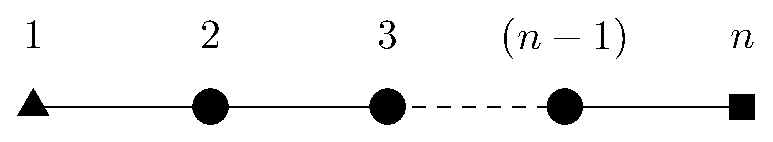
\includegraphics [scale=0.8] {images/1d}
    \caption{Область решения одномерной задачи теплопроводности.} 
    \label{images:1d}  
\end{figure}

Система линейных уравнений для МКЭ в матричной форме:

\begin{equation}
    K \overline{\psi} = \overline{b}
    \label{equ:slau}  
\end{equation}

где $K$ - матрица жесткости, $ \overline{\psi}$ - вектор неизвестных ячейковых температур в узлах, $ \overline{b}$ - вектор правой части.
Матрица жесткости имеет вид:

\begin{equation}
    K =
    \left(
        \begin{array}{cccccc}
            k_{1,1} & k_{1,2} & 0       & \ldots & 0           & 0         \\
            k_{2,1} & k_{2,2} & k_{2,3} & \ldots & 0           & 0         \\
            0       & k_{3,2} & k_{3,3} & \ldots & 0           & 0         \\
            \vdots  & \vdots  & \vdots  &        & \vdots      & \vdots    \\
            0       & 0       & 0       & \ldots & k_{n-1,n-1} & k_{n-1,n} \\
            0       & 0       & 0       & \ldots & k_{n,n-1}   & k_{n,n}   \\
        \end{array}
    \right)
    \label{equ:k1}  
\end{equation}

Коэффициенты $k_{1,2}$ и $k_{2,1}$ отражают взаимосвязь узлов $1$ и $2$, лежащих в пределах одного конечного эдементы, они не равны нулю. 
Коэффициенты $k_{1,n-1}$ и $k_{n-1,1}$ равны нулю, так как узлы $1$ и $n-1$ в разных конечных элементах. 
В матрице жесткости производятся следующие замены:

% \begin{equation}
%         \begin{array}{c}
%             k_{1,n-1} \leftarrow k_{n,n-1}, \\
%             k_{n-1,1} \leftarrow k_{n-1,N}, \\
%             k_{n,n-1} \leftarrow 0, \\
%             k_{n-1,n} \leftarrow 0, \\
%             k_{n,n}   \leftarrow 1
%         \end{array}
% \end{equation}

% \begin{equation}
        \begin{align*}
            k_{1,n-1} &\leftarrow k_{n,n-1}, \\
            k_{n-1,1} &\leftarrow k_{n-1,N}, \\
            k_{n,n-1} &\leftarrow 0, \\
            k_{n-1,n} &\leftarrow 0, \\
            k_{n,n}   &\leftarrow 1
        \end{align*}
% \end{equation}

получим матрицу такого вида:

\begin{equation}
    K^* =
    \left(
        \begin{array}{cccccc}
            k_{1,1}   & k_{1,2} & 0       & \ldots & k_{1,n-1}   & 0      \\
            k_{2,1}   & k_{2,2} & k_{2,3} & \ldots & 0           & 0      \\
            0         & k_{3,2} & k_{3,3} & \ldots & 0           & 0      \\
            \vdots    & \vdots  & \vdots  &        & \vdots      & \vdots \\
            k_{n-1,1} & 0       & 0       & \ldots & k_{n-1,n-1} & 0      \\
            0         & 0       & 0       & \ldots & 0           & 1      \\
        \end{array}
    \right)
    \label{equ:k2}  
\end{equation}

Вектор правой части остаётся неизменным.

Полученое уравнение (\ref{eq:new_K}) условно соответствует области решения в виде <<кольца>> (рис. \ref{images:1d_loop}).

\begin{equation}
    K^* \overline{\psi^*} = \overline{b}
    \label{eq:new_K}  
\end{equation}

\begin{figure} [ht]
    \center
    
\includegraphics [scale=0.8] {images/1d_loop}
    \caption{Области решения в виде <<кольца>>.} 
    \label{images:1d_loop}  
\end{figure}

После решения уравнения (\ref{eq:new_K}) производится обратная замена в векторе $\overline{\psi^*}$, что бы вернуть <<выброшенный>> граничный узел. 
Само решение получается с точностью до константы и на него налагается дополнительное условние, именуемое нормировки:

\begin{equation}
    \left< \Psi \right> = 0
\end{equation}

После нормировки решения $ \overline{\psi^*} $ получается $ \overline{\psi} $ , являющееся решение исходной системы уравнений \ref{equ:slau}. 

\textbf{Пример для случая 2-переодического композитного материала.} 
Задача имеет аналогичный вид задаче (\ref{equ:1d_beg})-(\ref{periodic_cell}) с той разницей что она поставленна для двумерной области решения. 
Пример сетки конечных элементов для двумерной ячейки периодичности представлен на рис. \ref{image:2d}.
Область разбита на четырёхугольные конечные элементы. 
Разбиение может иметь самый произвольный характер, за исключением граничных точек.
Граничные узлы должны быть расположенны симметрично, отночительно вертикальной и горизонтальной осей, проходящих через центр области.
Это означает что координаты $\xi_x$ узлов на левой грани должны совпадать с координатами $\xi_x$ аналогичных узлов правой грани.
То же для верхней и нижней граней, совпадение по координатам $\xi_y$.
На примере (рис.\ref{image:2d}) граничные узла расположенны равномерно, с постоянным шагом, но могут быть расположены и неравномерно.

\begin{figure} [ht] 
    \center
    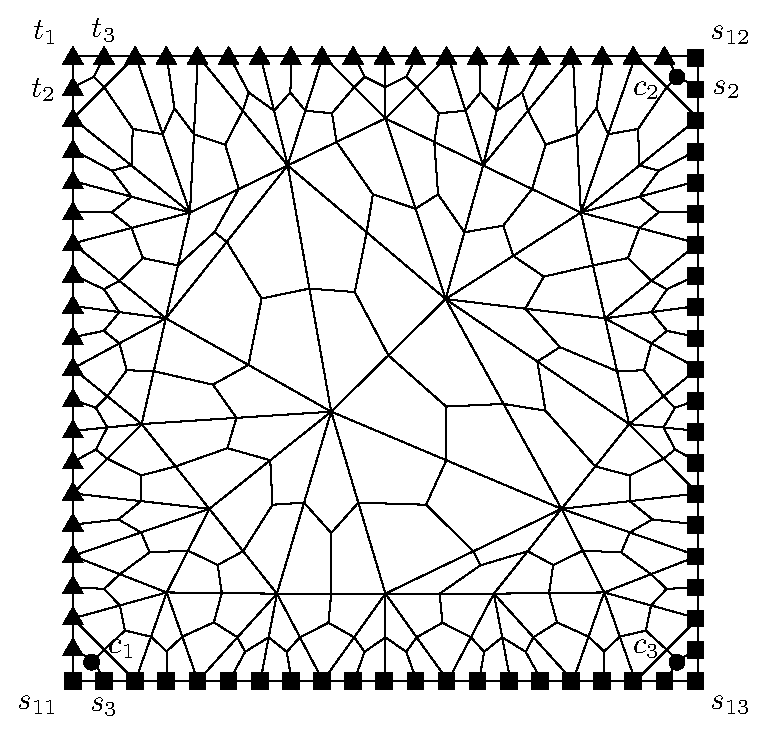
\includegraphics [scale=0.8] {images/2d}
    \caption{Область решения двумерной задачи теплопроводности.} 
    \label{images:2d}  
\end{figure}

С матрицей жесткости выполняются манипуляции аналогичные манипуляциям (\ref{equ:k1})-(\ref{equ:k2}), <<заменяются>> узлы, отмеченные квадратами (буква <<s>>),
на узлы, отмеченные треуголниками (буква <<t>>). Внутренние узлы на рис. \ref{image:2d} отмечены только в трёх точках, чтол бы не забивать изображение, и символьно обозначены буквами <<c>>.
Пример замены коэффициентов:

% \begin{equation}
%         \begin{array}{ccccc}
%             k_{t_1,c_1} = k_{s_{11},c_1},  k_{t_1,c_2} = k_{s_{12},c_2},  k_{t_1,c_3} = k_{s_{13},c_3},  k_{t_2,c_2} = k_{s_2,c_2},  k_{t_3,c_1} = k_{s_3,c_1}, \\
%             k_{s_{11},c_1} = 0,  k_{s_{12},c_2} = 0,  k_{s_{13},c_3} = 0,  k_{s_2,c_2} = 0,  k_{s_3,c_1} = 0, \\
%             k_{s_{11},s_{11}} = 1,  k_{s_{12},s_{12}} = 1,  k_{s_{13},s_{13}} = 1,  k_{s_2,s_2} = 1,  k_{s_3,s_3} = 1
%         \end{array}
% \end{equation}

\begin{align*}
    k_{t_1,c_1} &\leftarrow k_{s_{11},c_1}, & k_{t_1,c_2} &\leftarrow k_{s_{12},c_2}, & k_{t_1,c_3} &\leftarrow k_{s_{13},c_3}, & k_{t_2,c_2} &\leftarrow k_{s_2,c_2}, & k_{t_3,c_1} &\leftarrow k_{s_3,c_1}, \\
    k_{s_{11},c_1} &\leftarrow 0, & k_{s_{12},c_2} &\leftarrow 0, & k_{s_{13},c_3} &\leftarrow 0, & k_{s_2,c_2} &\leftarrow 0, & k_{s_3,c_1} &\leftarrow 0, \\
    k_{s_{11},s_{11}} &\leftarrow 1, & k_{s_{12},s_{12}} &\leftarrow 1, & k_{s_{13},s_{13}} &\leftarrow 1, & k_{s_2,s_2} &\leftarrow 1, & k_{s_3,s_3} &\leftarrow 1
\end{align*}

Замены для двумерной области решения в целом аналогичны заменам в одномерной, но есть особенность в угловых точках. 
Один уголовой узел $t_1$ <<заменяет>> все три остальных угловых узла: $s_{11}$, $s_{12}$, $s_{13}$.
После проведённых замен область решения станет соответствовать <<тору>>.

\textbf{Пример для случая 3-переодического композитного материала.} 
Задача имеет аналогичный вид задаче (\ref{equ:1d_beg})-(\ref{periodic_cell}) с той разницей что она поставленна для трёхмерной области решения. 
Пример сетки конечных элементов для двумерной ячейки периодичности представлен на рис. \ref{image:3d}.
Изображение плохо демонстрирует сетку, но не представляется возможным адекватно отобразить трёхмерную область на плоскость.
Область разбита на шестигранные объёмные конечные элементы. 
Разбиение может иметь самый произвольный характер, за исключением граничных точек.
Граничные узлы должны быть расположенны симметрично, отночительно трёх осей, проходящих через центр области.
Это означает что координаты $(\xi_x, \xi_y)$ узлов на одной грани должны совпадать с координатами $(\xi_x, \xi_y)$ аналогичных узлов на противоположной грани.
То же правило для двух остальных пар граней, с координатами $(\xi_x, \xi_z)$ и $(\xi_y, \xi_z)$.

\begin{figure} [ht] 
    \center
    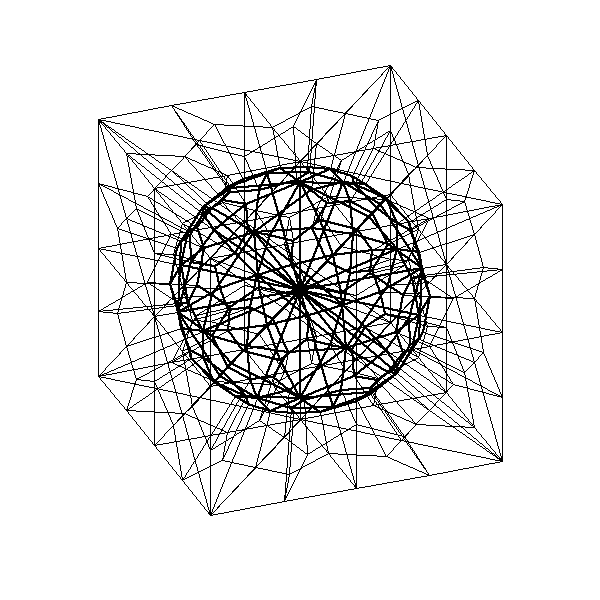
\includegraphics [scale=0.8] {images/3d}
    \caption{Область решения трёхмерной задачи теплопроводности.} 
    \label{images:3d}  
\end{figure}

С матрицей жесткости выполняются манипуляции аналогичные манипуляциям (\ref{equ:k1})-(\ref{equ:k2}).
Имеются особенности в угловый узлах и узлах на гранях. 
Один уголовой узел <<заменяет>> пять остальных угловых узлов. 
Узлы одного ребра заменяют соответствующие узлы остальных трёх рёбер, расположенных вдоль той же оси координат.


% \begin{equation*}
%     \left(
%         \begin{array}{*{13}c}
%              & \textcolor{blue}{B_1} & \ldots & \textcolor{blue}{B_2} & \ldots & \textcolor{red}{R_1} & \ldots & \textcolor{red}{R_2} & \ldots & D_1 & \ldots & D_2 & \ldots \\
%             \textcolor{blue}{B_1} & k_{B_1B_1} &  & k_{B_1B_2} &  & 0 &  & 0 &  & k_{R_1D_1} &  & k_{R_1D_2} &  \\
%             \vdots &  &  &  &  &  &  &  &  &  &  &  &  \\
%             \textcolor{blue}{B_2} & k_{B_1B_2} &  & k_{B_2B_2} &  & 0 &  & 0 &  & k_{R_2D_1} &  & k_{R_2D_2} &  \\
%             \vdots &  &  &  &  &  &  &  &  &  &  &  &  \\
%             \textcolor{red}{R_1} & 0 &  & 0 &  & 1 &  & 0 &  & 0 &  & 0 &  \\
%             \vdots &  &  &  &  &  &  &  &  &  &  &  &  \\
%             \textcolor{red}{R_2} & 0 &  & 0 &  & 0 &  & 1 &  & 0 &  & 0 &  \\
%             \vdots &  &  &  &  &  &  &  &  &  &  &  &  \\
%             D_1 & k_{R_1D_1} &  & k_{R_2D_1} &  & 0 &  & 0 &  & k_{D_1D_1} &  & k_{D_1D_2} &  \\
%             \vdots &  &  &  &  &  &  &  &  &  &  &  &  \\
%             D_2 & k_{R_1D_2} &  & k_{R_2D_2} &  & 0 &  & 0 &  & k_{D_1D_2} &  & k_{D_2D_2} &  \\
%             \vdots &  &  &  &  &  &  &  &  &  &  &  &  \\
%         \end{array}
%     \right)
% \end{equation*}






\end{document}
